\documentclass[tikz,border=10pt]{standalone}
\usepackage{tikz}
\usepackage{xcolor}
\usepackage{amsmath}

\tikzset{
  gauss/.style={draw, thick, domain=-1:1, smooth, variable=\x},
  arrow/.style={->, thick},
  label/.style={font=\small}
}

\begin{document}
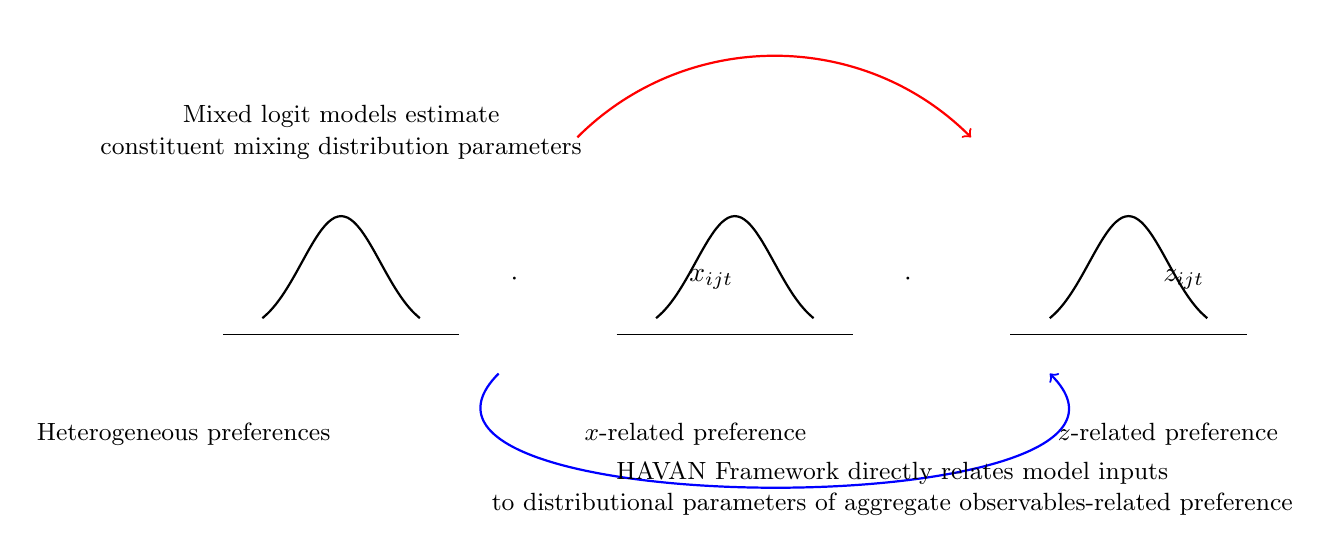
\begin{tikzpicture}[scale=1.0]

% Gaussian curves
\draw[gauss] plot (\x, {1.5*exp(-\x*\x*2)});
\draw[gauss] plot (\x+5, {1.5*exp(-\x*\x*2)});
\draw[gauss] plot (\x+10, {1.5*exp(-\x*\x*2)});

% Horizontal lines
\draw (-1.5,0) -- (1.5,0);
\draw (3.5,0) -- (6.5,0);
\draw (8.5,0) -- (11.5,0);

% Arrows
\draw[arrow, red] (3, 2.5) to [out=45,in=135] (8, 2.5);
\draw[arrow, blue] (2, -0.5) to [out=225,in=315] (9, -0.5);

% Labels
\node at (-2, -1) [label, below] {Heterogeneous preferences};
\node at (4.5, -1) [label, below] {$x$-related preference};
\node at (10.5, -1) [label, below] {$z$-related preference};
\node at (0, 2.5) [label, above] {Mixed logit models estimate};
\node at (0, 2.1) [label, above] {constituent mixing distribution parameters};
\node at (7, -1.5) [label, below] {HAVAN Framework directly relates model inputs};
\node at (7, -1.9) [label, below] {to distributional parameters of aggregate observables-related preference};

% Math symbols
\node at (2.2, 0.7) {$\cdot$};
\node at (7.2, 0.7) {$\cdot$};
\node at (4.7, 0.7) {$x_{ijt}$};
\node at (10.7, 0.7) {$z_{ijt}$};

\end{tikzpicture}
\end{document}